\documentclass[12pt,fleqn]{article}\usepackage{../../common}
\begin{document}
Evrişimsel Çizit Ağları (Graph Convolutional Networks)

Gerçek dünyadaki pek çok veriyi çizit olarak temsil etmek doğal; arkadaşlık
verisi, bilgi temsili. Çizitler bildiğimiz gibi düğümler ve o düğümler
arasındaki bağlantılardan oluşur, bilgi temsili örneğinde mesela A kişisi B
okulunda okudu için A ve B düğümleri arasında ``okudu'' bağlantısı konur,
ve yine bu kişinin C şehrinde ``yaşamış'' olduğu yine bir bağlantı ile
temsil edilebilir. Bu şekilde tüm çizit kurulabilir, ve sonra çizitin
özetsel bir halini hesaplattırabiliriz (temsili gömme verisi yaratmak
mümkün), sonra bu ``öğrenilmiş'' özet üzerinden eksik bilgileri çizite
sormak mümkün olabilir. Acaba A kişisi D işinde ``çalışmış mıdır?''. Bu
eksik bir bağlantı, belki veride yok ama olması gerekiyor, eldeki özetten
bu bilgi tamamlanabilir. 

Matematiksel olarak bir düğüm verisinin etrafındaki komşu düğümlerin bir
fonksiyonu olarak modellenir.

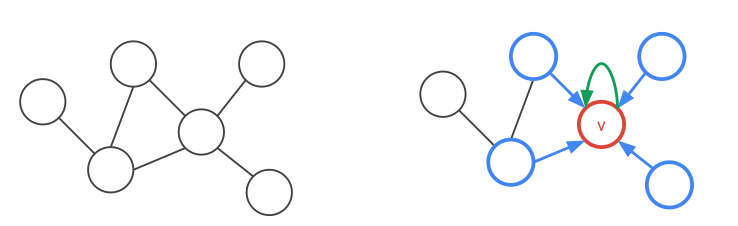
\includegraphics[width=30em]{graphconv_02.png}

Yaklaşıma evrişimsel denmesinin sebebi tüm 1. derece komşuluk ilişkilerinin
aynı ağırlıklar ile hesaplanıyor olması. Bu isim yaklaşımın ismi derin
yapay sinir ağlarındaki evrişimsel operatörlere benzemesinden geliyor, bir
evrişimsel operatörü veri üzerinde gezdirdiğimiz zaman o gezdirme
yapılırken operatörün hep aynı ağırlıkları kullanıldığı varsayarız / o
şekilde kodlarız.

$$ h_v = ReLU(W_{loop}h_v + \sum _{u \in N(v)} W h_u ) $$

$W_{loop}$ düğümlerin kendilerine olan bağlantısını (loop) modelliyor, buna
etraftaki bağlantılar ekleniyor. Fakat bir DYSA'da evrişimsel (ve diğer)
tabakalar, katmanlar vardır, GCN'de katmanlar nerede? Katmanlar bir düğümün
hesabı için kaç komşuluk seviyesi geriye gitmesi üzerinden
hesaplanıyor. Eğer bir düğüm için komşunun komşusuna gidiyorsak bu ilişki
ağın ikinci katmanını oluşturur.

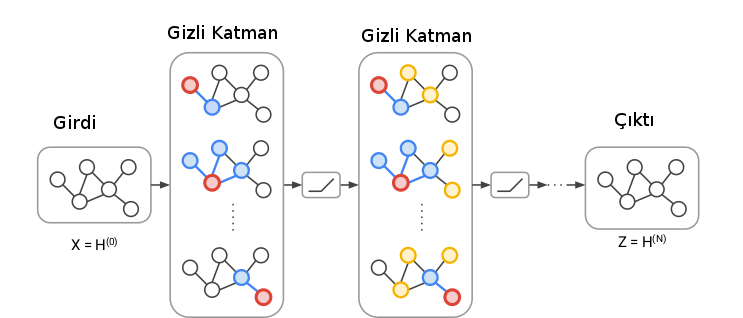
\includegraphics[width=35em]{graphconv_01.png}

Üstteki figürde gördüğümüz gibi ilk seviye komşuluklar mavi komşular ve
kırmızı düğüm arasında, bu birinci katman (her kırmızı düğüm için komşuluk
aynı ağırlıklarla). İkinci katmanda komşunun komşusu sarı düğümler de dahil
ediliyor, ve bunlar da farklı (ama yine her ikinci seviye komşuluk için
aynı) ağırlıklarla hallediliyor.

GCN'lerin diğer çizit işleyen yaklaşımlara göre bir diğer avantajı hem
bağlantı yapısını, hem de düğümler üzerindeki referans bilgisini de (mesela
kişileri temsil eden düğümlerde yaş, cinsiyet gibi bilgiler)
kullanabilmesi. 

[2] konudaki yayınlardan biri, örnek olarak bilimsel yayınların
birbirini referansını analiz etmişler, ayrıca tavsiye sistemleriyle kendi
yaklaşımlarını yarıştırmışlar, sonuçlar oldukca iyi [3].

Kod

\inputminted[fontsize=\footnotesize]{python}{util.py}

\inputminted[fontsize=\footnotesize]{python}{train.py}

Peki bu metotu keşfedenler çizitleri evrişimsel kavramlarla bağlantılamak
istemişler? Bunun sebebi büyük bir ihtimalle mevcut DYSA hesaplayan kodlama
altyapısından faydalanmak istemeleri. DYSA hesaplamak için Tensorflow gibi
kütüphanelerden oluşan kuvvetli bir kod altyapısı var artık, eğer
problemimizi bu kütüphanelerin çözebileceği formlara sokabilirsek pek çok
yan faydayı bedava elde edebilmiş oluruz. 

Üstteki kodu \verb!train.py!'dan işletince sonucu göreceğiz, AUC yüzde 90
civarında olmalı.

[devam edecek]

Kaynaklar

[1] Titov, {\em Extracting and Modeling Relations with Graph Convolutional Networks}, \url{http://www.akbc.ws/2017/slides/ivan-titov-slides.pdf}

[2] Kipf, {\em Variational Graph Auto-Encoders}, \url{https://arxiv.org/abs/1611.07308}

[3] Kipf, {\em Implementation of Graph Auto-Encoders in TensorFlow}, \url{https://github.com/tkipf/gae}

\end{document}
